%
% $Id: SANDExampleReportstrict.tex,v 1.27 2009/04/30 23:15:05 rolf Exp $
%
% This is an example LaTeX file which uses the SANDreport class file.
% It shows how a SAND report should be formatted, what sections and
% elements it should contain, and how to use the SANDreport class.
% It uses the LaTeX report class and the strict option.
%
% Get the latest version of the class file and more at
%    http://www.cs.sandia.gov/~rolf/SANDreport
%
% This file and the SANDreport.cls file are based on information
% contained in "Guide to Preparing {SAND} Reports", Sand98-0730, edited
% by Tamara K. Locke, and the newer "Guide to Preparing SAND Reports and
% Other Communication Products", SAND2002-2068P.
% Please send corrections and suggestions for improvements to
% Rolf Riesen, Org. 9223, MS 1110, rolf@cs.sandia.gov
%
\documentclass[pdf,ps2pdf,12pt,report,strict,blank]{SANDreport}
\usepackage{pslatex}
\usepackage{mathptmx}	% Use the Postscript Times font
\usepackage[FIGBOTCAP,normal,bf,tight]{subfigure}
\usepackage[dvips,light,first,bottomafter]{draftcopy}
\draftcopyName{Sample, contains no OUO}{70}

% If you want to relax some of the SAND98-0730 requirements, use the "relax"
% option. It adds spaces and boldface in the table of contents, and does not
% force the page layout sizes.
% e.g. \documentclass[relax,12pt]{SANDreport}
%
% You can also use the "strict" option, which applies even more of the
% SAND98-0730 guidelines. It gets rid of section numbers which are often
% useful; e.g. \documentclass[strict]{SANDreport}



% ---------------------------------------------------------------------------- %
%
% Set the title, author, and date
%
    \title{Optika: A GUI Framework for Parametrized Applications (Report style, strict)}

    \author{Kurtis L. Nusbaum \\
	  Scalable Algorithms \\
	  Sandia National Laboratories\\
	  P.O. Box 5800\\
	  Albuquerque, NM 87185-9999 \\
	  klnusba@sandia.gov \\
	 }

    % There is a "Printed" date on the title page of a SAND report, so
    % the generic \date should generally be empty.
    \date{}


% ---------------------------------------------------------------------------- %
% Set some things we need for SAND reports. These are mandatory
%
\SANDnum{SAND2010-xxxx}
\SANDprintDate{July 2010}
\SANDrePrintDate{January 2006}
\SANDrePrintDate{February 2006}
\SANDrePrintDate{March 2006}
\SANDauthor{Kurtis L. Nusbaum}


% ---------------------------------------------------------------------------- %
% Include the markings required for your SAND report. The default is "Unlimited
% Release". You may have to edit the file included here, or create your own
% (see the examples provided).
%
% \include{MarkUR} % Not needed for unlimted release reports


% ---------------------------------------------------------------------------- %
% The following definition does not have a default value and will not
% print anything, if not defined
%
\SANDsupersed{SAND1901-0001}{January 1901}


% ---------------------------------------------------------------------------- %
%
% Start the document
%
\begin{document}
    \maketitle

    % ------------------------------------------------------------------------ %
    % An Abstract is required for SAND reports
    %
    \begin{abstract}
	In the field of scientific computing there are many specialized programs designed for specific applications 
in areas like biology, chemistry, and physics. These applications are often very powerful and extraodinarily 
useful in their respective domains. However, many suffer from a common problem: a poor user interface. Many 
of these programs are homegrown, and the concern of the designer was not ease of use but rather 
functionality. The purpose of Optika is to address this problem and provide a simple, viable solution. Using
only a list of parameters passed to it, Optika can dynamically generate a GUI. This allows the user to specify 
parameters values in fashion that is much more intuitive than the traditional "input decks" used by many 
parameterized scientific applications. By leverageing the power of Optika, these scientific applications 
will become more accessible and thus allow their designers to reach a much wider audience while requiring 
minimal extra development effort.

    \end{abstract}


    % ------------------------------------------------------------------------ %
    % An Acknowledgement section is optional but important, if someone made
    % contributions or helped beyond the normal part of a work assignment.
    % Use \section* since we don't want it in the table of context
    %
    \clearpage
    \chapter*{Acknowledgment}
	    Thanks to Dr. Mike Heroux and Jim Willenbring. Their mentoring
	has been crucial to the development of Optika. Also, many thanks
	to the entire Trilinos Community in which Optika has found a
	welcoming home.

    The format of this report is based on information found
    in~\cite{Sand98-0730}.



    % ------------------------------------------------------------------------ %
    % The table of contents and list of figures and tables
    % Comment out \listoffigures and \listoftables if there are no
    % figures or tables. Make sure this starts on an odd numbered page
    %
    \cleardoublepage		% TOC needs to start on an odd page
    \tableofcontents
    \listoffigures
    \listoftables


    % ---------------------------------------------------------------------- %
    % An optional preface or Foreword
    %\clearpage
    %\chapter*{Preface}
    %\addcontentsline{toc}{chapter}{Preface}
	%    Although staff members usually have only limited experience
    with dry-erase markers, and many even dispute their existence,
    it is worthwhile to be open minded and explore the possibilities.



    % ---------------------------------------------------------------------- %
    % An optional executive summary
    %\clearpage
    %\chapter*{Summary}
    %\addcontentsline{toc}{chapter}{Summary}
	%    Once a certain level of mistrust and skepticism has been
    overcome, dry-erase markers find many uses in todays science and
    engineering. In this report we explain some of the fundamental
    properties, dangers, and benefits of dry-erase markers. We then
    conclude with a few examples on how they can be used in daily
    activities at national Laboratories.



    % ---------------------------------------------------------------------- %
    % An optional glossary. We don't want it to be numbered
    \clearpage
    \chapter*{Nomenclature}
    \addcontentsline{toc}{chapter}{Nomenclature}
    \begin{description}
	\item[Dependency]
	    A relationship ship between to parameters in which the state
		or value of one parameter depends on the state or value of
		another.
	\item[Dependee]
		The parameter upon which another parameter state or value dependes.
	\item[Dependent]
		A parameter whose state or value is determined by another
		parameter.
	\item[Parameter]
	    An input needed for a program.
	\item[Parameter List]
	    A list of parameters and other parameter lists.
	\item[RCP]
	    Refernce counted pointer. RCPs refered to in this document reference the
		RCP class located in the Teuchos package of Trilinos.
	\item[Sublist]
	    A parameter list contained within another parameter list.
    \end{description}


    % ---------------------------------------------------------------------- %
    % This is where the body of the report begins; usually with an Introduction
    %
    \SANDmain		% Start the main part of the report

    \chapter{Introduction}
	\label{Intro}
	This report is comprised of two main sections. The first section discusses the development
of Optika. Design choices and problems that arrised during development are
discussed in this section. The second section is intended to be a manual on how to use
Optika. If the reader desires simple to learn how to use Optika, it is suggested he/she
skip to the second section.



    \chapter{Development of the Optika package}
	This section of the report discusses the developement of the Optika package.

\section{Initial Planning}
In Fall of 2008. Dr. Mike Heroux identified a need for
the Trilinos framework to include some sort of GUI package. Dr. Heroux wanted 
to give users of the framework the ability to easily generate GUIs for their
programs, while still providing a good experience for the end user. Based on
previous GUI work done for the Tramonto project, a few initial problems were
identified:

	\begin{itemize}
		\item How would the GUI be laid out?
		\item Different types of parameters require different methods of input.
			How would we decide how we would obtain input for a particular
			parameter?
		\item What framework would we use to build the GUI?
		\item How would the application developer specify parameters for the
			GUI to obtain?
		\item How would the application developer specify dependencies between
		parameters. This was a crucial problem/needed feature that was identified in
		development of the Tramonto GUI.
	\end{itemize}

After some deliberation, the following initial solutions were decided upon:

	\begin{itemize}
		\item The GUI would be laid out in a hierarchical fashion as shown in
		Figure \ref{paramlistFigure}. Parameters organized into lists and sublists. This
		would allow for a clear organization of the parameters as well as
		intrinsically demonstrate the relationships between them.
		\begin{figure}
			\centering
			\begin{picture}(50,150)(0,0)
				\put(10,0){\line(0,1){145}}
				\put(0,150){${Parameter List}$}
				\put(10,130){\line(1,0){15}}
				\put(28,127){$Parameter$}
				\put(10,110){\line(1,0){15}}
				\put(28,107){$Parameter$}
				\put(10,90){\line(1,0){15}}
				\put(28,87){$Parameter$}
				\put(10,70){\line(1,0){15}}
				\put(28,67){$Parameter List$}
				\put(38,0){\line(0,1){62}}
				\put(38,47){\line(1,0){15}}
				\put(56,44){$Parameter$}
				\put(38,22){\line(1,0){15}}
				\put(56,24){$Parameter$}
			\end{picture}
			\caption[GUI Layout]{The hierarchical layout of the GUI}
			\label{paramlistFigure}
		\end{figure}
		\item It be required that all parameters specify their type and the
		following types would be accepted:
			\begin{itemize}
				\item int
				\item short
				\item float
				\item double
				\item string
				\item boolean
				\item arrays of int, short, double, and string
			\end{itemize}
		For number types, a spin box would be used as input. If the valid
		values for a string type were specified, a combo box would be used.
		Otherwise a line edit would be used. For booleans, a combo box would
		also be used. For arrays, a pop-up box containing numerous input
		widgets would be used. The widget type would be determined by the
		array type.
		\begin{figure}[h]
			\centering
			\subfigure[A Spin Box]{
				\label{spinboxfig}
				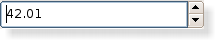
\includegraphics[scale=0.5]{graphics/spinbox}
			}
			\subfigure[A Combo Box]{
				\label{comboboxfig}
				
\includegraphics[scale=0.5]{graphics/combobox}
			}
			\subfigure[A Line Edit]{
				\label{lineeditfig}
				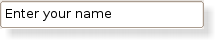
\includegraphics[scale=0.5]{graphics/lineedit}
			}
			\caption{Some of the various widgets used for editing data}
			\label{editingWidgets}
		\end{figure}

		\item QT was chosen as the GUI framework for several reasons:
			\begin{itemize}
				\item It is cross-platform.
				\item It is mature and has a well developed set of
				development tools.
				\item It has a rich feature-set.
				\item It has been used by Sandia in the past.
				\item The Optika developer was familiar with it.
			\end{itemize}
		\item Initially it was decided that the application developer would
		specify parameters via an XML file. A DTD would be created specifying
		the legal tags and name spaces.
		\item Dependencies would be handled through special tags in the DTD.
	\end{itemize}

\section{Early Development}
The first several months of development were spent on creating and implementing the XML
specification. The name of the XML specification went through several revisions but was
eventually called Dependent Parameter Markup Language (DPML).

After several months of development it was realized that creating an entirely new way of specifying 
parameters might hinder it's adoption. It pointed out that Trilinos actually had
a ParameterList~\cite{ParameterList} class in the Teuchos package. The ParameterList semmed to be better than DPML for
several reasons:
	\begin{itemize}
		\item It was already heavily adopted.
		\item It had the necessary hierarchical nature.
		\item It was serializable to and from XML.
	\end{itemize}

For these reasons, DPML was scrapted in favor of using Teucho's ParameterLists. Development moved
forward with the goal of creating a GUI framework that, in addiiton to meeting all the challenges 
outlined above, would also be compatiable with any existing program using Teuchos's ParameterLists.

\section{Heavy development}
Starting in May 2009 a more heavy focus was put on developement of the Trilinos GUI package.
With the backend data-structure of the Teuchos's ParameterList already in place, attention
was turned to the developing the actually GUI itself. A key technology provided by Qt was it's Model/View
framework~\cite{QtModelView}. Using the Model/View paradigm, a wrapper class named TreeModel
~\cite{TreeModel} was created around the ParameterList class by subclassing the 
QAbstractItemModel~\cite{QAbstractItemModel}.

However, in subclassing the QAbstractItemModel it was realized that the ParameterList class fell short in
certain areas. At this point the main issue was that a given ParameterEntry~\cite{ParameterEntry} located within
a ParameterList or a given sublist located within a ParameterList was not aware of it's parent.
This was an issue because Qt's Model/Veiw framework requires items within a model to be aware of
their parents. In order to circumvent this issue the TreeItem~\cite{TreeItem} class was created. Now 
instead of simply wrapping around a ParameterList class, the TreeModel created by giving it a ParameterList.
It would then read in the ParameterList and creat a structure of TreeItems.  Each TreeItem then contained a pointer 
to it's corresponding ParameterEntry.

Once the TreeModel and TreeItem class were complete an appropriate delegate to go between and View
and the TreeModel was needed. A new class called Delegate~\cite{Delegate} was created to fill this
role by subclassing QItemDelegate~\cite{QItemDelegate}. As specified above, the delegate would return
the apporiate editing widget based on it's datatype.

With the model and delegate classes inplace, an appropriate view could be applied. At first a simple
QTreeView~\cite{QTreeView} was applied to the model. The results was something like that in \ref{treeviewFig}.
	\begin{figure}[h]
		\centering
			\subfigure[A Tree View]{
				\label{treeviewFig}
				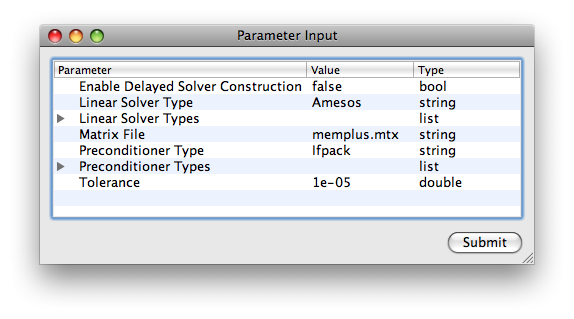
\includegraphics[scale=0.5]{graphics/treeview}
			}
	\end{figure}





    \chapter{A Long Chapter}\label{sec:long}
	    We need a long chapter to test full-page formatting. Therefore,
    we switch to the ancient language of Latin.

    %
% Generated by http://www.lipsum.com
% I could have used the LaTeX package lipsum.sty, but it is not present in all
% LaTeX distributions and would make the examples less portable.
%
Lorem ipsum dolor sit amet, consectetuer adipiscing elit. Maecenas ante augue, dictum ut, scelerisque vitae, sagittis vel, velit. Curabitur velit. Curabitur eleifend eleifend felis. Curabitur purus. Nunc aliquet felis a pede. Suspendisse dictum consequat nunc. In accumsan. Sed sit amet diam. Aliquam rhoncus, orci non sodales suscipit, libero risus condimentum lacus, vitae laoreet velit purus ac est. Etiam id sem eu arcu pellentesque rhoncus. Quisque feugiat est at elit lacinia vestibulum. Integer eget nisl sed diam sodales egestas.

Quisque risus libero, pellentesque ac, iaculis a, pulvinar quis, leo. Cras sapien erat, lacinia sit amet, accumsan porta, bibendum malesuada, nulla. Suspendisse non lorem. Sed pellentesque nulla id nisl. In hac habitasse platea dictumst. Ut nec sem. Proin interdum fringilla felis. Aenean lacus. Quisque nisi. Aliquam congue venenatis purus. Vestibulum ante ipsum primis in faucibus orci luctus et ultrices posuere cubilia Curae; Suspendisse a nunc.

Nunc lobortis. Aliquam ultricies volutpat felis. Nulla nisi tellus, ultrices vel, sodales in, lacinia at, leo. Fusce odio turpis, mattis nec, semper ut, aliquam nec, odio. Sed tristique lacus eget arcu. In at elit. Duis semper, est ut sagittis tempor, risus arcu mattis ligula, quis posuere velit ipsum a neque. Proin mattis, urna vehicula tempus placerat, nisl tortor pharetra dolor, nec luctus orci nisi a ante. Ut a lectus at nulla ultricies congue. Ut rhoncus, purus in malesuada rhoncus, nisi ante laoreet lectus, eget volutpat dui nunc ac metus. Sed dignissim faucibus elit. Vestibulum cursus nonummy mauris. Vestibulum dapibus neque eu ligula. Ut scelerisque urna ut orci tincidunt volutpat. Aliquam ipsum purus, eleifend sed, nonummy non, dapibus vel, metus. Class aptent taciti sociosqu ad litora torquent per conubia nostra, per inceptos hymenaeos.

Ut vitae mauris. Aenean diam. Nam euismod massa bibendum orci. Proin sed arcu. Phasellus commodo lacus. Nunc sit amet dolor eget arcu iaculis congue. Sed volutpat, dolor nec porta facilisis, purus mi euismod lacus, sed pharetra magna arcu id dolor. Vestibulum a purus nec nisl varius facilisis. Sed semper mattis lorem. Suspendisse tellus dolor, tincidunt fermentum, imperdiet eu, ultrices et, massa. Nulla facilisi. Nulla rhoncus. Ut vestibulum quam feugiat quam. Aliquam nisi. Vivamus facilisis euismod ipsum. Nunc suscipit semper felis. Nunc non metus. Vestibulum ante ipsum primis in faucibus orci luctus et ultrices posuere cubilia Curae;

Maecenas posuere rutrum odio. Curabitur dolor quam, semper sed, malesuada eu, sagittis eu, erat. Vestibulum facilisis, ipsum vitae venenatis consectetuer, ipsum nibh scelerisque lacus, quis nonummy elit augue et lectus. Fusce ut dolor et ligula laoreet commodo. Phasellus ornare. Aliquam erat volutpat. Ut sapien leo, auctor vel, placerat vel, pretium quis, libero. Integer tempus interdum tellus. Vestibulum posuere, mi ultricies ullamcorper ornare, dolor nunc condimentum tellus, et commodo neque tellus at mi. Aliquam porttitor, tortor eu interdum malesuada, justo nisl feugiat lacus, eu venenatis augue tortor sit amet arcu. Maecenas quis enim. Mauris fringilla diam. Maecenas vitae metus a felis ullamcorper vestibulum. Suspendisse potenti. Etiam sit amet elit. Ut iaculis risus in odio.

Quisque porttitor, velit at consectetuer pretium, nibh lacus dignissim erat, id imperdiet tellus lectus vel sapien. Integer varius dignissim urna. Vestibulum elementum lobortis lorem. Morbi vel metus in risus consectetuer facilisis. Quisque ac purus eget ipsum interdum semper. Suspendisse blandit, nisi in mattis condimentum, elit sem tempus dui, eu convallis mi dolor in dui. Nunc vehicula eros in diam. Sed lectus velit, varius ut, posuere eget, lacinia a, augue. Suspendisse odio lectus, tincidunt porttitor, porttitor vitae, rhoncus id, turpis. Sed quam. Duis tortor tortor, ultrices ut, imperdiet a, convallis a, magna. Donec pellentesque sapien vitae elit. Fusce egestas eleifend velit. Pellentesque habitant morbi tristique senectus et netus et malesuada fames ac turpis egestas.

Proin ac sapien. Aenean tincidunt ante aliquet tortor. In non elit nec tortor pharetra pretium. Nulla facilisi. Maecenas pulvinar odio in libero. Nam tincidunt nulla et dui. Nunc in eros nec dolor congue varius. Suspendisse euismod. Aliquam nulla nibh, vulputate in, molestie ut, suscipit quis, orci. Ut feugiat sapien id velit. Nullam rutrum, enim non dictum posuere, nulla diam faucibus risus, vel suscipit tellus nisi nec libero. Nullam scelerisque vestibulum sem.

Sed ultrices ligula vel lacus. Donec elit felis, venenatis volutpat, varius eu, placerat cursus, sem. Nullam non felis quis enim laoreet dictum. Nulla in nisl at erat pretium facilisis. Vestibulum sed ante. In hac habitasse platea dictumst. Aenean lobortis ullamcorper ante. Aenean at magna. Etiam viverra erat id augue. Morbi purus. Sed congue. Integer sit amet enim vel sapien ullamcorper auctor. Phasellus neque sapien, cursus sit amet, pharetra ac, mollis non, nibh. Ut risus orci, dignissim eu, feugiat sit amet, ullamcorper sit amet, tortor. Nunc ac ligula ut libero fermentum tincidunt. Morbi lorem metus, bibendum ut, aliquet at, tristique vulputate, nisl. Duis risus turpis, bibendum in, faucibus cursus, eleifend sit amet, erat. Donec elit purus, facilisis nec, vulputate non, gravida et, eros. Curabitur porttitor sapien ac magna. Donec cursus.

Cras sodales posuere pede. Lorem ipsum dolor sit amet, consectetuer adipiscing elit. Donec id nisi eu erat tempus ornare. Ut diam magna, bibendum sit amet, porttitor tempor, malesuada non, tellus. Duis iaculis gravida ante. Morbi dapibus elementum orci. Donec eget metus. Curabitur varius tortor condimentum nunc. In arcu. Nam ante justo, porta sed, pellentesque vitae, tristique in, metus. Nam ultricies nulla quis tellus. Donec egestas enim et dolor. In ornare ligula et eros.

Proin augue ligula, dictum non, viverra vitae, convallis sed, ipsum. Maecenas vitae justo. Lorem ipsum dolor sit amet, consectetuer adipiscing elit. Aliquam erat volutpat. Aenean eget ligula. Nullam id dui eu lacus euismod iaculis. Nulla erat purus, convallis ac, ullamcorper a, vestibulum id, erat. Sed pulvinar consectetuer neque. Nulla lobortis. Nulla congue, sapien in hendrerit rhoncus, est sem dignissim mauris, non nonummy nunc justo volutpat velit. Quisque suscipit risus a ipsum mattis viverra. Pellentesque habitant morbi tristique senectus et netus et malesuada fames ac turpis egestas. Vestibulum ante ipsum primis in faucibus orci luctus et ultrices posuere cubilia Curae; Fusce libero dolor, aliquam vel, varius id, faucibus sollicitudin, massa.

Proin iaculis semper ligula. Pellentesque malesuada, neque sit amet ornare mattis, augue lacus auctor tellus, quis porttitor felis sapien a nibh. In sed orci. Pellentesque congue purus sit amet urna. Proin tincidunt molestie nibh. Nulla et dui ac turpis venenatis ullamcorper. Nunc at nisl. Pellentesque habitant morbi tristique senectus et netus et malesuada fames ac turpis egestas. Cum sociis natoque penatibus et magnis dis parturient montes, nascetur ridiculus mus. Sed magna. Curabitur gravida, metus id semper interdum, dui orci ullamcorper massa, congue ornare mauris lectus rhoncus mi. Integer justo ante, sollicitudin tempor, egestas sit amet, egestas eu, eros. Etiam leo. Integer tristique velit nec nunc.

Nulla ac nibh id nunc volutpat ultrices. Lorem ipsum dolor sit amet, consectetuer adipiscing elit. Praesent a arcu. Suspendisse blandit justo eu justo. Nunc turpis metus, iaculis eget, molestie eu, egestas hendrerit, nibh. Sed elementum placerat metus. Cras pretium turpis non ipsum. Duis in libero. Praesent ut elit eu magna tempus rhoncus. Nunc consectetuer quam ac orci. In nulla.

Donec porta turpis a velit. Donec accumsan. Pellentesque augue magna, cursus sed, elementum eget, cursus id, enim. Duis purus. Suspendisse tristique. Quisque condimentum. Quisque tristique lacus vitae nulla. Nunc nibh velit, gravida et, placerat nec, feugiat sed, ante. Phasellus nisi. Aenean auctor pede at leo. Nullam semper fringilla dui. Quisque est. Suspendisse dolor sem, euismod ac, tempor vitae, nonummy id, felis. Mauris eu tellus. Morbi rhoncus. Cum sociis natoque penatibus et magnis dis parturient montes, nascetur ridiculus mus. Nam sed nisi. Fusce ac sapien sit amet arcu venenatis facilisis. Proin faucibus pharetra risus.

Sed varius elit vitae urna. Ut at felis. Phasellus euismod metus a ante. Suspendisse eu massa. Nullam bibendum dui pulvinar turpis. Mauris lacinia odio id augue. Morbi ligula. Nulla ac massa. Nullam vel arcu. Pellentesque iaculis, tellus et convallis condimentum, erat diam viverra nibh, eget pellentesque mauris lorem faucibus neque.

Curabitur tincidunt, dui ac dictum iaculis, enim magna porttitor orci, quis ullamcorper enim magna commodo justo. Aliquam ut quam in velit porta consequat. Suspendisse potenti. Nunc cursus rutrum eros. Curabitur varius molestie massa. Fusce accumsan fringilla sem. Pellentesque habitant morbi tristique senectus et netus et malesuada fames ac turpis egestas. In hac habitasse platea dictumst. Pellentesque risus nisl, tincidunt sed, sodales ac, interdum ac, diam. In purus ipsum, porttitor feugiat, viverra ac, mattis eget, ligula. Sed bibendum libero in metus. Morbi ornare. Donec libero justo, fringilla vitae, mollis sit amet, molestie ut, mauris. Morbi vel dolor. Donec at elit eget metus semper pharetra. Morbi est massa, volutpat ut, viverra varius, sagittis blandit, sapien. Sed dapibus. Pellentesque erat. Nullam hendrerit. Vestibulum vel diam in tortor consectetuer volutpat.

Quisque accumsan, elit quis sodales pellentesque, sapien metus consequat enim, et commodo leo nulla in elit. Donec varius. Donec ut risus. Donec quis lacus quis nisi congue consectetuer. In sed odio. Duis nulla sem, ullamcorper ac, suscipit dignissim, suscipit vel, turpis. Fusce suscipit. Maecenas in augue non felis fermentum luctus. Aenean sem. Etiam in leo sit amet tortor malesuada auctor. Curabitur quis massa. Maecenas aliquam lectus. Maecenas sit amet augue. Sed sem elit, egestas vitae, condimentum suscipit, elementum et, nulla. Lorem ipsum dolor sit amet, consectetuer adipiscing elit. Nam dignissim tristique velit.

Pellentesque dui elit, tristique non, cursus a, elementum sed, magna. Ut eu augue. Maecenas scelerisque lectus vel enim. Vivamus eu mauris. Phasellus venenatis. Maecenas egestas. Phasellus ac purus. Sed vel dui. Nam consectetuer venenatis lacus. Morbi ullamcorper, urna ac viverra tempor, urna dui imperdiet dui, sit amet hendrerit elit nisi ac lorem. Nullam gravida diam ut tellus. Aenean quam tortor, condimentum ac, commodo non, pharetra in, elit. Mauris tincidunt, orci sit amet lacinia varius, diam tortor dapibus tellus, id scelerisque quam magna pharetra libero. Curabitur aliquet, ante sit amet ornare volutpat, urna ipsum dictum ipsum, at ullamcorper ligula arcu eget leo.

Ut libero lorem, condimentum nec, rhoncus id, vestibulum a, nisl. Cras hendrerit euismod sapien. Sed lectus ipsum, vehicula et, luctus vitae, venenatis at, magna. Ut nec nisl in quam facilisis tincidunt. Fusce enim purus, pellentesque vitae, molestie ut, dapibus in, eros. Integer eu turpis vel pede volutpat posuere. Nam porttitor suscipit metus. Curabitur mollis, quam quis porttitor nonummy, libero ante pulvinar magna, a bibendum massa erat nec sapien. Donec ac turpis. Suspendisse elit nisi, ultrices ut, fringilla sed, vestibulum suscipit, mauris. Cum sociis natoque penatibus et magnis dis parturient montes, nascetur ridiculus mus. Phasellus dictum aliquam lacus. Praesent in erat quis nunc consectetuer dictum. Morbi dignissim, turpis ut varius pharetra, tellus lectus rutrum lacus, bibendum iaculis velit nulla ac orci. Etiam gravida nibh eget massa. Sed elementum convallis purus. Duis tincidunt feugiat lacus. Donec id enim nec enim ullamcorper condimentum. Suspendisse urna.




    \chapter{Conclusion}
	    Of course, no report would be complete without some conclusions.
    This section is where they would go, if we had any.


    \nocite{*}


    % ---------------------------------------------------------------------- %
    % References
    %
    \clearpage
    % If hyperref is included, then \phantomsection is already defined.
    % If not, we need to define it.
    \providecommand*{\phantomsection}{}
    \phantomsection
    \addcontentsline{toc}{chapter}{References}
    \bibliographystyle{plain}
    \bibliography{SANDExample}


    % ---------------------------------------------------------------------- %
    %
    \appendix
    \chapter{Historical Perspective}
	    This is an example of an appendix.

    If we follow~\cite{Sand98-0730} strictly, we would have to have
    a separate bibliography section for each appendix.  The style
    file doesn't provide that, but it can be done using the {\tt
    bibunits} and {\tt chapterbib} packages.

    If there are many subsections in an appendix, it should also
    have its own table of contents. Again, the SAND report class
    file does not provide that functionality.

    \ifthenelse{\boolean{reportSAND}}   {
	\section{The Past a Long Time Ago}
    }{
	\subsection{The Past a Long Time Ago}
    }
	This is where we talk about things so old nobody can verify
	them. We are safe.

    \ifthenelse{\boolean{reportSAND}}   {
	\section{The Past More Recently}
    }{
	\subsection{The Past More Recently}
    }
	Now we have to be a little bit more careful, since records
	exist from that time, and some people still alive actually
	lived back then.



    \chapter{Some Other Appendix}
	    Just to show what a second Appendix would look like. It contains
    a table. Each appendix is supposed to be self-contained, so
    tables and figures are not supposed to show up in the main
    table of contents. There can be a separate table of contents
    for each appendix.

    \begin{table}[ht]
	\centering
	\caption{A small table}
	\bigskip

	\begin{tabular}{|c|c|}
	    \hline
		A & B  \\ \hline
		C & D  \\ \hline
	\end{tabular}
	\label{tab3}
    \end{table}

    \begin{figure}[ht]
	\centering
	\begin{picture}(50,50)(0,0)
	    \put(25,25){\circle{1}}
	    \put(25,25){\circle{5}}
	    \put(25,25){\circle{10}}
	    \put(25,25){\circle{15}}
	    \put(25,25){\circle{20}}
	    \put(25,25){\circle{25}}
	    \put(25,25){\circle{30}}
	    \put(25,25){\circle{35}}
	    \put(25,25){\circle{40}}
	    \put(25,25){\circle{45}}
	    \put(25,25){\circle{50}}
	\end{picture}
	\caption{Dizzy yet?}
	\label{fig4}
    \end{figure}


    % \printindex

    %
% This is an example of how to create the distribution page. Some
% distributions are required by Sandia; e.g. the housekeeping copies.
% Depending on the type of report; e.g. CRADA, Patent Caution, etc.
% additional distribution lines may have to be added. See the
% "Guide for Preparing SAND Reports"
%

{\bfseries DISTRIBUTION}

{\bfseries Email--External (encrypt for OUO)}\\[1ex]
\begin{tabular}{|p{4cm}|p{5cm}|p{4cm}|}
  \hline
  \multicolumn{1}{|>{\centering\arraybackslash}p{4cm}|}{\cellcolor{SANDgreen}\bfseries Name} & \multicolumn{1}{>{\centering\arraybackslash}p{5cm}|}{\cellcolor{SANDgreen}\bfseries Company Email Address} & \multicolumn{1}{>{\centering\arraybackslash}p{4cm}|}{\cellcolor{SANDgreen}\bfseries Company Name}\\
  \hline
  Matthias Mayr & matthias.mayr@unibw.de & University of the Bundeswehr Munich\\
  \hline
  Andrey Prokopenko & prokopenkoav@ornl.gov & Oak Ridge National Laboratory\\
  \hline
  Tobias Wiesner & tobias.wiesner@leica-geosystems.com & Leica Geosystems AG\\
  \hline
\end{tabular}

{\bfseries Email--Internal}\\[1ex]
\begin{tabular}{|p{5cm}|p{3cm}|p{5cm}|}
  \hline
  \multicolumn{1}{|c}{\cellcolor{SANDgreen}\bfseries Name} & \multicolumn{1}{|c}{\cellcolor{SANDgreen}\bfseries Org.} & \multicolumn{1}{|c|}{\cellcolor{SANDgreen}\bfseries Sandia Email Address}\\
  \hline
  Luc Berger-Vergiat & 1442 & lberge@sandia.gov\\
  \hline
  Christopher Siefert & 1465 & csiefer@sandia.gov\\
  \hline
  Christian Glusa & 1465 & caglusa@sandia.gov\\
  \hline
  Mark Hoemmen & 1541 & mhoemme@sandia.gov\\
  \hline
  Jonathan Hu & 1465 & jhu@sandia.gov\\
  \hline
  Paul Lin & 1422 & ptlin@sandia.gov\\
  \hline
  Ray Tuminaro & 1442 & rstumin@sandia.gov\\
  \hline
  Technical Library & 9536 & libref@sandia.gov\\
  \hline
\end{tabular}


    % The second printing
    \begin{SANDreDistribution}
	% Some external Addresses
	\SANDdistExternal{1}{An Address\\ 99 $99^{th}$ street NW\\City, State}
	\SANDdistExternal{3}{Some Address\\ and street\\City, State}
	\SANDdistExternal{12}{Another Address\\ On a street\\City, State\\U.S.A.}
	\bigskip


	% Internal Addresses
	\SANDdistInternal{1}{1319}{Rolf Riesen}{1423}

	% Example of a mail channel use (instead of a mail stop)
	\SANDdistInternalM{1}{M9999}{Someone}{01234}
    \end{SANDreDistribution}

    % The third printing
    \begin{SANDreDistribution}
	\SANDdistInternal{1}{1319}{Rolf Riesen}{01423}
    \end{SANDreDistribution}

    % The fourth printing
    \begin{SANDreDistribution}
	\SANDdistInternal{1}{1319}{Rolf Riesen}{1423}
    \end{SANDreDistribution}

\end{document}
